% Please use the skeleton file you have received in the 
% invitation-to-submit email, where your data are already
% filled in. Otherwise please make sure you insert your 
% data according to the instructions in PoSauthmanual.pdf
\documentclass{PoS}

\usepackage{subfigure}
% \usepackage{cite} --> non fa vedere i link
% \usepackage{hyperref} --> non funziona

\newcommand{\ptjet}{\ensuremath{{p}_{T}^{\mathrm jet}}}
\newcommand{\antikt}{anti-$k_t$}

\title{Searches for Heavy Hadronic Resonances with the ATLAS and CMS detectors at the LHC}

\ShortTitle{Hadronic resonances at the LHC}

\author{\speaker{Caterina Doglioni, Francesco Santanastasio}\\%\thanks{A footnote may follow.}\\
        University of Geneva and CERN\\
        E-mail: \email{caterina.doglioni@cern.ch}, \email{francesco.santanastasio@cern.ch}}

% \author{\speaker{Francesco Santanastasio}\\
%        CERN\\
%        E-mail: \email{francesco.santanastasio@cern.ch}}
% 
\abstract{This review focuses on a series of searches for new resonances decaying to hadronic final states in the ATLAS and CMS experiments. 
Searches for dijet resonances, R-Parity Violating SUSY gluinos and resonances decaying in boosted top pairs and heavy bosons using jet substructure techniques
are outlined, and differences between the search strategies of the two experiments are highlighted. Issues relevant for measurements to be performed with the increased center-of-mass and luminosity at the LHC after 2015 are also raised for further discussion.}

\FullConference{VI Italian workshop on p-p physics at the LHC,\\
		8-10 May 2013\\
		Acquario di Genova, Ponte Spinola, Area Porto Antico, Genova, Italy}


\begin{document}

\section{Introduction}
New resonances, coupling to quarks and gluons and decaying to hadronic final states, 
can be produced copiously at the Large Hadron Collider (CERN). 
%The large cross section of processes decaying in quarks and gluons 
%at the Large Hadron Collider makes searches for new, heavy resonances decaying 
%into hadronic jets an attractive ground to test the validity of the Standard Model 
%to the highest energy scales. 
This review outlines a selection of searches for heavy resonances in hadronic final states 
performed at the ATLAS and CMS experiments using LHC proton-proton collision data collected 
at a center-of-mass energy of 7 TeV (2011) and 8 TeV (2012). A series of points that 
are deemed important for current and future searches are also discussed.

%\section{Jet reconstruction and calibration: da tagliare?}

%Both ATLAS and CMS employ similar algorithms and techniques for jet reconstruction, 
%as most searches employ the \antikt{} jet finding algorithm~\cite{Cacciari:2008gp},
%although the inputs for jet finding are different. ATLAS uses energy deposits from the calorimeters,
%while CMS complements the calorimeter information with measurements of particle momenta
%from the inner detector. The hadronic energy scale is calibrated using a series of corrections 
%derived both from Monte-Carlo simulation and from 
%data~\cite{ATLAS-CONF-2013-004, 1748-0221-6-11-P11002, Aad:2011he}. 
%The jet energy scale uncertainty, which dominates among the sources of systematic 
%uncertainty for most of the searches described in this review, is derived using data-driven 
%techniques and has a similar magnitude across
%jet transverse momenta $p_\mathrm{T}$ and pseudorapidities $\eta$ for the two experiments. 
%However, as it can be noted in Figure~\ref{Fig:JESUnc}, 
%the estimate of the uncertainty for jets above 2~TeV differs between ATLAS and CMS.  

%\begin{figure}[b]
%\subfigure[ATLAS jet energy scale uncertainty]
%{\includegraphics[width=0.58\textwidth]{Figure/ATLASJES.pdf}}
%\subfigure[CMS jet energy scale uncertainty]
%{\includegraphics[width=0.4\textwidth]{Figure/CMSJES.png}}
%\caption{Typical jet energy uncertainties for central jets in ATLAS and CMS.}
%\label{Fig:JESUnc}
%\end{figure}

\section{Overview of selected searches in the ATLAS and CMS experiments}

The searches for hadronic resonances can be divided in two main categories:
\begin{itemize}
 \item {\bf Resolved topology} - Searches where the quarks and gluons produced in the final state are reconstructed at detector level into single,  \textit{resolved} hadronic jets. Examples are the single production of a resonance X decaying to a pair of gluons, or the pair production of two resonances X at rest each decaying to a quark-antiquark pair;
 \item {\bf Boosted topology} - Searches where the quarks and gluons produced in the final state are merged into a single reconstructed jet.  A typical example is the decay of a resonance X into a pair of massive particles Y, with $\mbox{M}_{X} >>\mbox{M}_{Y} $, and Y decays to a pair of light quarks. In this case the resonance Y will be \textit{boosted} 
(the resonance has a large momentum compared to its mass) so that a single hadronic jet with a large distance 
parameter encompasses all its decay products. Techniques that exploit the presence of substructure within this jet are employed to reject background from standard QCD jets and reduce the dependence on multiple interactions within the same bunch crossing (pile-up). 
\end{itemize}

The quintessential example of hadronic search with resolved jets is the 
search for heavy resonances in the dijet mass distribution. New particles, 
or excitations of quarks indicating 
compositeness,
%further substructure
could manifest 
themselves as narrow 'bumps' in the dijet mass distribution of central leading
and subleading jets above the continuum QCD background~\cite{CMS-PAS-EXO-12-059, ATLAS-CONF-2012-148}. 
The search can be tailored to specific resonances
decaying to heavy quark flavors using $b-$tagging for one or both jets~\cite{CMS-PAS-EXO-12-023}. 
No significant excess over the background has been found in the current ATLAS and CMS searches,
and lower limits are set on the masses of new particles 
%(Fig.~\ref{Fig:DijetRes}~(a)), 
including model-independent Gaussian resonances of varying width.
%(Fig.~\ref{Fig:DijetRes}~(b)). 
Upper limits of the order of $100$, $10$ and $1$~fb at are set on cross section times branching fraction to jets times acceptance 
for resonance masses of 1.5, 3, and 4.5 TeV, respectively.

%\begin{figure}[t]
%\subfigure[CMS limits for various resonances]
%{\includegraphics[width=0.48\textwidth]{Figure/DijetCMS.pdf}}
%\subfigure[ATLAS limits on Gaussian resonances]
%{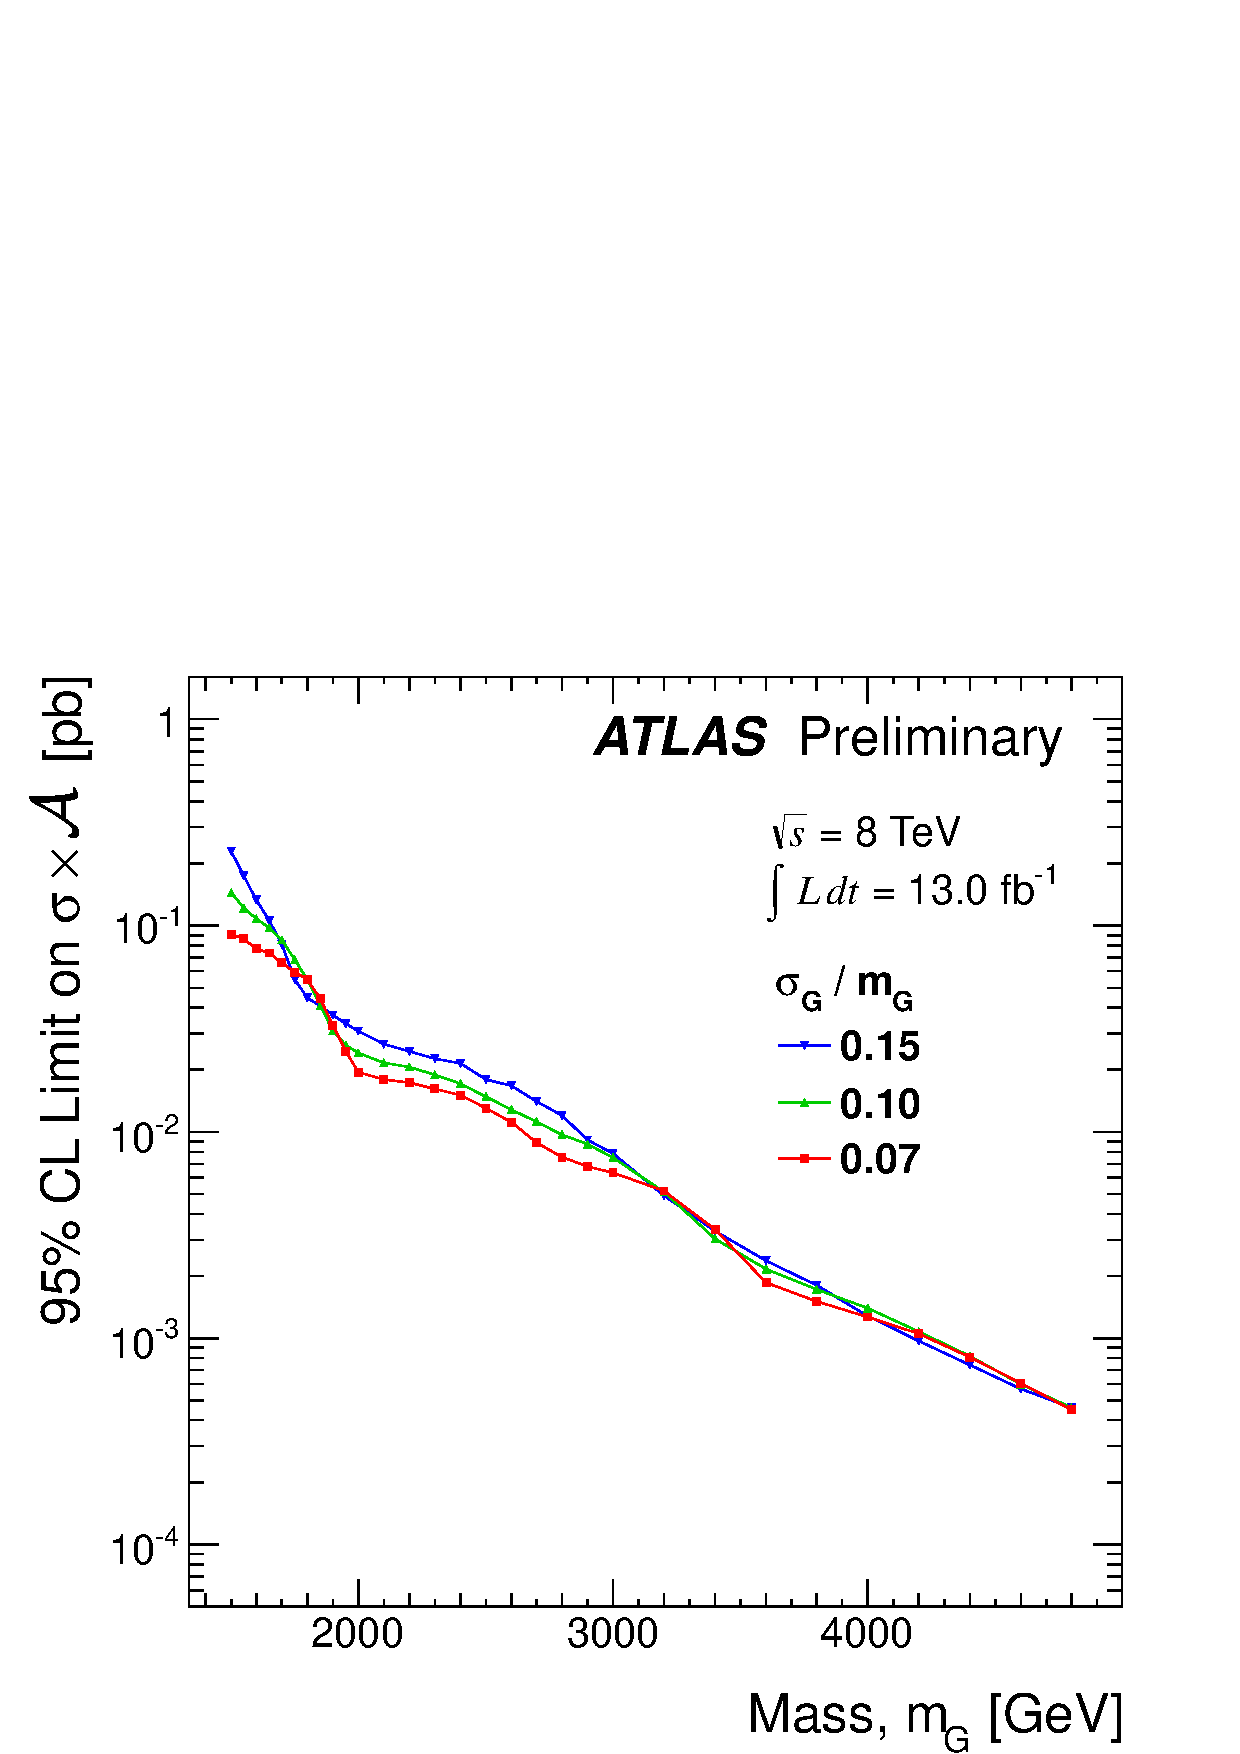
\includegraphics[width=0.48\textwidth]{Figure/DijetGaussATLAS.pdf}}
%\caption{95\% CL limits from dijet mass resonance searches.}
%\label{Fig:DijetRes}
%\end{figure}

Searches for resonances in final states with high jet multiplicity, optimized for R-Parity Violating supersymmetric 
signatures (3-body decays into quarks of pair produced gluinos, giving a six jet final state), 
can be performed in both resolved and boosted regimes~\cite{Chatrchyan2012329,SUSYRPVATLAS}.
Both experiments select events with six or more jets, but the background estimation techniques differ in
ATLAS and CMS. In the resolved channel, ATLAS employs the $p_\mathrm{T}$
of the sixth jet as a discriminant variable, while CMS performs a 'bump-hunt' in the 
three-jet invariant mass. The combinatorial background (from both the QCD background and the signal)
penalizes the CMS search and allows the ATLAS search to set more stringent limits. A proof-of-principle
boosted-jet analysis, although not as sensitive as the resolved one, is also carried out by the ATLAS experiment~\cite{SUSYRPVATLAS}. 
 
In the case of resonances decaying into pairs of top quarks ($\mbox{t}\bar{\mbox{t}}$) or heavy bosons (e.g. WW, ZZ, HH, HZ, ..), 
the use of jet substructure techniques is crucial to achieve a good background rejection. 
In these cases, the top quarks or heavy bosons coming from a TeV-scale resonance 
would be boosted, and therefore their decay products would be spatially collimated in the detector.  

Specific techniques for top-tagging, based on the presence of three hard energy deposit corresponding
to the top decay products, have been employed to distinguish top-jets from jets originated from quarks and gluons
that constitute the majority of the QCD background~\cite{Kaplan:2008ie, Plehn:2010st, ATLAS-CONF-2012-065, Almeida:2010pa}. 
Both ATLAS and CMS look for heavy resonances decaying in $t\bar{t}$ in both 7 and 8 TeV data, 
in semileptonic and all-hadronic top decays~\cite{TtbarResCMS, TtbarResATLAS, CMS-PAS-B2G-12-005, ATLAS-CONF-2013-052, CMS-PAS-B2G-12-006}.
The ATLAS analysis employs $b-$tagging to further suppress the QCD background and sets limits starting from a resonance mass of 500 GeV. 
The CMS analysis, instead, does not use $b-$tagging and limits are set starting at a resonance mass of 1 TeV. 
In the case of the 7 TeV analysis, the CMS expected upper limits on the resonance cross section are 
about a factor 3-4 lower than the ATLAS ones 
for resonance masses around 2 TeV.  The top-tagging technique (requiring the presence of $b-$tagged jets) used
by ATLAS allows the search to start at lower resonance masses 
compared to CMS, by reducing significantly the QCD background.
On the other hand, the low b-tag efficiency at high jet $ p_\mathrm{T}$ and the more conservative
treatment of uncertainties could reduce the sensitivity of the ATLAS search at high resonance masses.

The CMS experiment has also performed a search for RS gravitons decaying to 
WW/ZZ and W'/Z' decaying to Wq/Zq~\cite{Chatrchyan:2012ypy}. This analysis employs 
W/Z-tagging techniques based on the jet mass and the presence
of hard sub-jets to significantly reduce the background, while keeping a relatively high signal efficiency. 
Given no excesses above background, limits are set on a number benchmark models. 

\section{Discussion points}

\subsection{Jet energy scale in ATLAS and CMS}

Resolved searches in ATLAS and CMS employ the \antikt{} jet finding algorithm~\cite{Cacciari:2008gp}.
% The inputs for jet finding are different: ATLAS uses energy deposits from the calorimeters,
% while CMS complements the calorimeter information with measurements of particle momenta
% from the inner detector. 
The hadronic energy scale is calibrated using a series of corrections 
derived from both Monte-Carlo simulation and from 
data~\cite{ATLAS-CONF-2013-004, 1748-0221-6-11-P11002, Aad:2011he}. 
The jet energy scale uncertainty, which dominates among the sources of systematic 
uncertainty for most of the searches described in this review, is derived using data-driven 
techniques and has a similar magnitude across
jet transverse momenta $p_\mathrm{T}$ and pseudorapidities $\eta$ for the two experiments. 
However, 
%as it can be noted in Figure~\ref{Fig:JESUnc}, 
the estimate of the uncertainty for jets above 2~TeV differs between ATLAS and CMS. 
This is mostly due to different assumptions made beyond the
$p_\mathrm{T}$ reach of the $in-situ$ calibration techniques. ATLAS employs conservative
uncertainties of particles beyond the range of test beam data ($p>$350 GeV)~\cite{Aad:2012vm} 
which lead to an uncertainty as high as 10\% for high-momentum particles within jets, 
while CMS uses a flat 3\% uncertainty for all particle types and momenta~\cite{CMS-PAS-JME-10-008}. 
Further discussion on this point would allow to adopt a coherent treatment for 
the most relevant uncertainty for hadronic searches between the two experiments,
paving the way for possible combinations of the result. 

\subsection{Setting limits on dijet resonances}

The search for hadronic resonances in the dijet mass spectrum presents 
the following~differences in the jet reconstruction and the 
limit-setting procedure between the two experiments:
\begin{itemize}
\item ATLAS uses \antikt{} jets with distance parameter equal to 0.6 (AK6), while 
CMS starts from  \antikt{} jets with distance parameter 0.5
(AK5) and then clusters AK5 jets within $\Delta\mbox{R}=\sqrt{\Delta\phi^2+\Delta\eta^2}=1.1$ around the 
two leading jets, to form two wide jets. This is done to recover energy from final 
state radiation.
 \item CMS uses the Narrow Width Approximation to define the resonance cross-section and signal template, 
while ATLAS employs the full simulated template without any truncation;
 \item the CMS limit is restricted to dijet final states (setting limits 
on cross-section times acceptance times branching ratio), while the ATLAS search is 
inclusive and would include in its acceptance e.g. photons from excited quarks 
as they are reconstructed as jets. 
\end{itemize}
Even though there are no important differences between the mass limits obtained by the two searches, 
it would be desirable to unify the definitions of one of the benchmark searches for New Phenomena at the LHC
for future iterations and possible combinations. 

\subsection{Trigger strategy for low-mass resonances}
In absence of evidence for new physics at the TeV scale so far, 
searching for new, low cross-section resonances in hadronic final states with masses 
between the electroweak ($\approx$ 100 GeV) and the TeV scale, 
becomes increasingly important for the experimental and the theory community.
Due to the steady increase of instantaneous luminosity of the LHC and to 
the large rates of final states containing jets, 
the trigger thresholds for hadronic triggers are now significantly 
higher compared to the LHC startup in 2010. As an example, the 2010 
dijet search with the first 3 pb$^{-1}$ of data could be performed 
starting from a dijet mass of $\approx$ 200 GeV, 
while the same analysis performed in 2012 
could only start at $\approx$ 1 TeV due to the high 
prescales of lower jet $p_\mathrm{T}$ triggers.

In addition to the regular developments for the "core" physics triggers, the 
ATLAS and CMS experiments have implemented two complementary trigger and data 
acquisition strategies to mitigate the problem of increased 
hadronic trigger rate in high luminosity scenarios.
\begin{itemize}
\item {\bf ATLAS Delayed Streams and} {\bf CMS Data Parking}~\cite{CMS-DP-2012-022} - 
The "core" physics program of ATLAS and CMS  at 8 TeV uses data collected
at the average event rate of few hundred Hz (for an average instantaneous luminosity of 
$\approx 4 \cdot 10^{33} \mbox{cm}^{-2}\mbox{s}^{-1}$). 
The "core" data are promptly reconstructed (within a few days) and are available during data taking. 
Additional data (about a factor of 2) have been collected by both experiments 
to extend the physics programs, both in terms of Standard Model (SM) 
measurements and beyond-SM (BSM) searches. 
These new triggers can be implemented as either a looser version of the core triggers
or as brand new triggers with small overlap with the rest. 
The additional data are reconstructed after the end of 8 TeV data 
taking (delayed reconstruction), as soon as the computing resources become available.
\item {\bf CMS Data Scouting}~\cite{CMS-DP-2012-022} - The idea beyond this novel approach 
is to collect pp collision events with very low trigger thresholds (such as $p_\mathrm{T}$ sum 
of jets in the event above 250 GeV) at a high rate (order of kHz) 
to extend the sensitivity to low-mass resonances decaying to final 
states with jets. This is possible only because a reduced event content 
is stored (for instance only calorimeter jets reconstructed during the High Level Trigger processing). 
No raw data from the detector channels are stored, and therefore the offline reconstruction 
is not possible in this special stream. However, thanks to the reduced per-event size, 
the data acquisition bandwidth (rate $\times$ event size) can be kept
under control. This approach was successfully tested by CMS at the end of 2011, 
and lead to an improvement in the limits on low-mass dijet resonances~\cite{CMS-PAS-EXO-11-094}. 
These triggers were also enabled during 2012 and the analyses of these data 
are currently ongoing. The continuous monitoring of this special data stream during the 
data taking would provide the possibility of dynamically extending the standard trigger 
setup, both for core physics and for special triggers, in case unexpected phenomena appear. 
\end{itemize}

%\begin{itemize}
%\item One/two-sentence description of need to look lower in mjj, hadronic rate problems, delayed triggers and parked data
%\item one plot only: CMS 2011 low-mass extension
%\end{itemize}

\subsection{New directions in searches with jet substructure}

Searches for heavy resonances X that decay to massive particles Y 
(such as the top quark, W, Z, or H in the SM), with Y decaying in hadrons, have been also 
considered in the discussion. The Lorentz factor $\gamma$ (boost factor) of the resonance 
Y is approximately $\mbox{M}_{X} / 2 \mbox{M}_{Y}$~\cite{Gouzevitch:2013qca}. 
Due to the kinematics of the event, a large boost factor implies 
that the decay products will be predominantly merged into a single reconstructed jet (the $\Delta R$ between the decay 
products is of the order of $2 \mbox{M}_{Y} / p_\mathrm{T}^{Y}$~\cite{ATLAS-CONF-2012-065}). 
When searching for resonances X with a mass greater than $\approx 1.5$~TeV, 
the use of jet substructure techniques becomes mandatory to identify the dominant
hadronic boosted decays of massive SM particles Y. 
Therefore, ATLAS and CMS experiments should invest 
in the study of substructure techniques in view of the startup at 14 TeV 
center-of-mass energy. Those techniques could benefit the 
searches of new resonances, as well as the measurement of 
WW scattering at high~$\sqrt{s}$. 

Much of the success of these searches will depend on the understanding of jet substructure 
and of jet grooming techniques at high jet $p_\mathrm{T}$. Grooming techniques such as trimming~\cite{Trimming}
or pruning~\cite{Ellis:2009me,Ellis:2009su} 
are used to reduce the dependence of jet 
internal properties from pile-up and non-perturbative physics, by rejecting low $p_\mathrm{T}$ 
and large-angle jet constituents during the jet re-clustering process.
%Studies on how to improve both the rejection of extra energy coming from particles extraneous to the hard scattering
%and the modelling of softer jets physics need to be undertaken before data taking resumes. 
Current studies~\cite{ATLAS-CONF-2012-066} show that these algorithms work well in 
presence of multiple interactions, up to 30 pile-up events. 
These studies should be extended to cover the 50 and 100 pile-up 
interaction scenarios which we expect to face in the 
14 TeV data taking.

The MC modeling of the jet substructure variables and backgrounds to searches in 
the boosted regime could also be improved in 
view of the aforementioned searches. 
SM measurements could provide a more precise description of the 
QCD-like backgrounds, and help reducing the systematic uncertainties 
related to the top-tagging and W/Z-tagging efficiency.
8 TeV data are available to proceed with MC tuning work, 
and the two experiments could already 
agree upon a certain set of benchmark observables and techniques to 
be investigated, e.g. using jet mass measurements 
for different jet grooming algorithms~\cite{Chatrchyan:2013rla,ATLAS:2012am}.

Jet substructure is currently a very active field both in terms of theoretical development and in experimental implementation.
To conclude, we report below two ideas for future applications of jet substructure methods in the LHC analyses which 
were discussed during the workshop:
\begin{itemize}
% \item {\bf N-subjettiness} - A promising jet substructure observable, which have been recently started to be used in both
% ATLAS and CMS, is the {\it N-subjettiness}~\cite{Stewart:2010tn,Thaler:2010tr,Thaler:2011gf}. 
% This observable quantities the compatibility of a jet with the hypothesis that it is 
% formed by "N" main sub-structures (for example N$=$2 could identify two quarks from a W decay), 
% by exploiting the $p_\mathrm{T}$ of the jet constituents and the $\Delta R$ between the jet constituents and 
% the "N" axes representing the hypothesized subjets. The ratio of 
% {\it N1-subjettiness} and {\it N2-subjettiness} is a powerful discriminator between jets containing "N1" and "N2" sub-structures. 
\item  {\bf Jet charge} - The idea of using of a weighted sum of the charges of the constituents of a jet, to distinguish 
among jets with different charges, have been recently discussed in the context of the LHC~\cite{Krohn:2012fg}.
Potential applications include measuring electroweak quantum
numbers of hadronically-decaying resonances or supersymmetric particles, as well as 
Standard Model tests, such as jet charge in dijet events or in hadronically-decaying W 
bosons in top-antitop pair events.
\item {\bf Energy and angular resolution of subjets} - We consider a massive, boosted SM particle Y (for example a W) 
decaying to a pair of quarks that merge into a single reconstructed jet with a large distance parameter. 
The reconstruction of the 4-momenta of the two subjets within this jet is important if one wants to 
measure the polarization of the particle Y in boosted regime. One important application is the WW scattering 
at large invariant mass of the diboson system, where the goal is to isolate the longitudinal scattering 
amplitude from the transverse one, as highlighted in Ref.~\cite{Han:2009em}.
To accomplish this task the energy and angular resolution of subjets 
should be studied in detail, as well as their dependence on the momentum of the particle Y and on the pileup environment. 
\end{itemize}

%\begin{itemize}
%\item New ideas:
%\begin{itemize}
 %\item Q/g tagging for lower masses
% \item Tools for W' and Z': jet charge and angle between subjets (angular correlations?)
%\end{itemize}
%\item Open questions:
%\begin{itemize}
% \item Particle flow and substructure
%\item High-lumi and substructure
%\end{itemize}
%\end{itemize}

\section{Acknowledgments}
The authors wish to thank the organizers of the "VI Italian workshop on p-p physics at the LHC" 
for the invitation and the for the rich and interesting physics program.

\bibliographystyle{JHEP}
\bibliography{skeleton}

% \begin{thebibliography}{99}
% 
% \bibitem{CMS-PAS-JME-10-008}
% Single-particle response in the CMS calorimeters.
% \newblock CMS-PAS-JME-10-008, CERN, Geneva, 2010.
% 
% \bibitem{ATLAS-CONF-2012-065}
% Performance of large-R jets and jet substructure reconstruction with the ATLAS
%   detector.
% \newblock ATLAS-CONF-2012-065, CERN, Geneva, Jul 2012.
% 
% \bibitem{ATLAS-CONF-2012-148}
% Search for new phenomena in the dijet mass distribution updated using 13.0
%   fb$^{-1}$ of $pp$ collisions at $sqrt{s}=8$ TeV collected by the ATLAS
%   detector.
% \newblock ATLAS-CONF-2012-148, CERN, Geneva, Nov 2012.
% 
% \bibitem{ATLAS-CONF-2013-004}
% Jet energy scale and its systematic uncertainty in proton-proton collisions at
%   $sqrt{s}$=7 tev with ATLAS 2011 data.
% \newblock ATLAS-CONF-2013-004, CERN, Geneva, Jan 2013.
% 
% \bibitem{CMS-PAS-B2G-12-005}
% Search for anomalous top quark pair production in the boosted all-hadronic
%   final state using pp collisions at sqrt(s) = 8 tev.
% \newblock CMS-PAS-B2G-12-005, CERN, Geneva, 2013.
% 
% \bibitem{CMS-PAS-EXO-12-023}
% CMS Collaboration
% \newblock
% Search for heavy resonances decaying into bb and bg final states in pp
%   collisions at sqrt(s) = 8 tev.
% \newblock Technical Report CMS-PAS-EXO-12-023, CERN, Geneva, 2013.
% 
% \bibitem{CMS-PAS-EXO-12-059}
% CMS Collaboration
% \newblock Search for narrow resonances using the dijet mass spectrum with 19.6fb-1 of pp
%   collisions at sqrts=8 tev.
% \newblock Technical Report CMS-PAS-EXO-12-059, CERN, Geneva, 2013.
% 
% \bibitem{ATLAS:2012am}
% ATLAS Collaboration
% \newblock {Jet mass and substructure of inclusive jets in $\sqrt{s}=7$ TeV $pp$
%   collisions with the ATLAS experiment}.
% \newblock {\em JHEP}, 1205:128, 2012.
% 
% \bibitem{Aad:2011he}
% Georges Aad et~al.
% \newblock {Jet energy measurement with the ATLAS detector in proton-proton
%   collisions at $\sqrt{s}=7$ TeV}.
% \newblock {\em Eur.Phys.J.}, C73:2304, 2013.
% 
% \bibitem{Aad:2012vm}
% Georges Aad et~al.
% \newblock {Single hadron response measurement and calorimeter jet energy scale
%   uncertainty with the ATLAS detector at the LHC}.
% \newblock {\em Eur.Phys.J.}, C73:2305, 2013.
% 
% \bibitem{Almeida:2010pa}
% Leandro~G. Almeida, Seung~J. Lee, Gilad Perez, George Sterman, and Ilmo Sung.
% \newblock {Template Overlap Method for Massive Jets}.
% \newblock {\em Phys.Rev.}, D82:054034, 2010.
% 
% \bibitem{Cacciari:2008gd}
% Matteo Cacciari, Juan Rojo, Gavin~P. Salam, and Gregory Soyez.
% \newblock {Quantifying the performance of jet definitions for kinematic
%   reconstruction at the LHC}.
% \newblock {\em JHEP}, 0812:032, 2008.
% 
% \bibitem{Chatrchyan:2012ypy}
% Serguei Chatrchyan et~al.
% \newblock {Search for heavy resonances in the W/Z-tagged dijet mass spectrum in
%   pp collisions at 7 TeV}.
% \newblock 2012.
% 
% \bibitem{Chatrchyan:2013rla}
% Serguei Chatrchyan et~al.
% \newblock {Studies of jet mass in dijet and W/Z+jet events}.
% \newblock 2013.
% 
% \bibitem{SUSYRPVATLAS}
% The~ATLAS Collaboration.
% \newblock Search for pair production of massive particles decaying into three
%   quarks with the ATLAS detector in $\sqrt{s}=7\;\mathrm{TeV}$ pp collisions at
%   the lhc.
% \newblock {\em Journal of High Energy Physics}, 2012(12):1--42, 2012.
% 
% \bibitem{TtbarResATLAS}
% The~ATLAS Collaboration.
% \newblock Search for resonances decaying into top-quark pairs using fully
%   hadronic decays in pp collisions with ATLAS at $\sqrt{s}$=7 tev.
% \newblock {\em Journal of High Energy Physics}, 2013(1):1--50, 2013.
% 
% \bibitem{1748-0221-6-11-P11002}
% The~CMS collaboration.
% \newblock Determination of jet energy calibration and transverse momentum
%   resolution in CMS.
% \newblock {\em Journal of Instrumentation}, 6(11):P11002, 2011.
% 
% \bibitem{TtbarResCMS}
% The~CMS Collaboration.
% \newblock Search for anomalous $t\overline t$ production in the highly-boosted
%   all-hadronic final state.
% \newblock {\em Journal of High Energy Physics}, 2012(9):1--41, 2012.
% 
% \bibitem{Chatrchyan2012329}
% The~CMS Collaboration.
% \newblock Search for three-jet resonances in pp collisions at.
% \newblock {\em Physics Letters B}, 718(2):329 -- 347, 2012.
% 
% \bibitem{Kaplan:2008ie}
% David~E. Kaplan, Keith Rehermann, Matthew~D. Schwartz, and Brock Tweedie.
% \newblock {Top Tagging: A Method for Identifying Boosted Hadronically Decaying
%   Top Quarks}.
% \newblock {\em Phys.Rev.Lett.}, 101:142001, 2008.
% 
% \bibitem{Plehn:2010st}
% Tilman Plehn, Michael Spannowsky, Michihisa Takeuchi, and Dirk Zerwas.
% \newblock {Stop Reconstruction with Tagged Tops}.
% \newblock {\em JHEP}, 1010:078, 2010.
% 
% \end{thebibliography}

\end{document}


